\documentclass[UTF8]{ctexart}
\usepackage{graphicx}
\usepackage{listings}
\usepackage{hyperref}
\usepackage{xcolor}
\usepackage{amsmath}
\newtheorem{corollary}{Corollary}[section]

\title{位运算问题整理}
\author{seeker}
\date{\today}	

\lstset{
	basicstyle          =   \sffamily,          % 基本代码风格
	keywordstyle        =   \bfseries,          % 关键字风格
	commentstyle        =   \rmfamily\itshape,  % 注释的风格,斜体
	stringstyle         =   \ttfamily,  % 字符串风格
	flexiblecolumns,                % 别问为什么,加上这个
	numbers             =   left,   % 行号的位置在左边
	showspaces          =   false,  % 是否显示空格,显示了有点乱,所以不现实了
	numberstyle         =   \zihao{-5}\ttfamily,    % 行号的样式,小五号,tt等宽字体
	showstringspaces    =   false,
	captionpos          =   t,      % 这段代码的名字所呈现的位置,t指的是top上面
	frame               =   lrtb,   % 显示边框
}

\lstdefinestyle{cpp}{
	language        =   C++, % 语言选Python
	basicstyle      =   \zihao{-5}\ttfamily,
	numberstyle     =   \zihao{-5}\ttfamily,
	breaklines      =   true,   % 自动换行,建议不要写太长的行
	columns         =   fixed,  % 如果不加这一句,字间距就不固定,很丑,必须加
	basewidth       =   0.5em,
}

\begin{document}
	\maketitle
	\begin{abstract}
		本篇讲义收集了若干codeforces上的位运算问题,通过分析题目的方式,加深信息学竞赛选手位运算的理解。
	\end{abstract}
	\section{引言}
	位运算问题通常伴随着与(AND)、或(OR)、异或(XOR)运算,且以异或运算为主(记作$\oplus$),由于其模型较为单一,涉及到的知识较少,通常以思维题的形式出现,通过位运算题目训练,可以较好的提升选手的问题转化与建模能力。
	
	本文通过一些位运算题目,探讨一些思维构造性问题,帮助选手深入理解位运算。
	\section{\href{https://codeforces.com/problemset/problem/1775/B}{Gardener and the Array}}
	\subsection{题目大意}
	给定数组$c$,定义$$f(c)=c_1|c_2|...|c_n$$其中,$|$表示或运算(OR),是否存在$c$的子数组$a$、$b$,使得$f(a)=f(b)$。
	\subsection{数据范围}
	$n$表示数组$c$的大小,$n\in(1,1e5)$,$c_i\in(1,2^{1e5})$
	\subsection{解题过程}
	考虑到$f(c)$涉及按位或运算,因此将$c_i$化为二进制的形式。
	
	由于子数组$a$,$b$不同的定义为存在不同元素,所以可以考虑使$a$,$b$包含大部分相同元素,只存在一个不同元素,考虑到
	$f(a)\leq  f(c)$,可以令$a=c$,即寻找是否存在元素$c_i$,使得
	$$f(c-c_i)=f(c)$$
	为了满足上述式子,$c_i$二进制位中每一位为1的位,在数组$c$中不能是唯一置1的,否则删去$c_i$后不能满足上式。
	在实际实现中还需要注意清空数组问题。
	\subsection{参考代码}
	\lstinputlisting[
	style       =   cpp,
	caption     =   {Gardener and the Array参考代码},
	label       =   {problem1.cpp}
	]{problem1.cpp}
	
	
	\section{\href{https://codeforces.com/problemset/problem/1742/G}{Orray}}
	\subsection{题目大意}
	给定长度为$n$的非负数组$a$,定义
	$$b_i=a_1|a_2|...|a_i$$
	试对着$a$重新排序,使得生成的数组$b$字典序最大。
	
	注:当数组$x$字典序大于$y$时,$x$和$y$中第一个不相同的位置$i$,满足$x_i\textgreater y_i$。
	\subsection{数据范围}
	$n\in [1,2\cdot 10^5]$,$a_i\in [0,10^9]$
	\subsection{解题过程}
	为了使得字典序最大,第一个$ans_1$值一定是$a$中最大值。那么,为了让第二个$ans_2$值最大,需要使得除了$ans_1$置一位以外的位尽可能的大。因此,等同于在减去$ans_1$的置一位后的数组中寻找最大值,由此得到第二个$ans_2$值。
	
	剩下的答案可以以此类推,即:在剩余数组中寻找并输出最大值->通过减去最大值的置一位更新剩余数组。这种方法看似是$O(N^2)$,但由于每个数据位最多被删去一次,因此在删去全部的数据位后,剩余的数组就全是0了,可以将剩下的$a$直接输出了,实际复杂度是$O(NlogN)$。
	
	\subsection{参考代码}
	\lstinputlisting[
	style       =   cpp,
	caption     =   {Orray参考代码},
	label       =   {problem2.cpp}
	]{problem2.cpp}
	
	\section{\href{https://codeforces.com/problemset/problem/1731/C}{Even Subarrays}}
	\subsection{题目大意}
	给定长度为$n$的数组$a$,计算数对$(i,j)$的数量,满足
	$$x=a_i\oplus a_{i+1}\oplus ...\oplus a_j$$,其中$x$是有偶数个因子数字。
	\subsection{数据范围}
	$$n\in [2,2\cdot10^5],a_i\in [1,n]$$
	\subsection{解题过程}
	首先考虑满足偶数因子的数字问题,由于一个非1数字的因子至少包含$1$和其本身,所以有奇数个因子的数字一定是是完全平方数。
	
	本题转换为,计算有多少对数对的异或和是完全平方数,由于$a_i\in [1,2\cdot10^5]$,所以其异或和得到的完全平方数小于262144,可以预处理1000多个完全平方数。
	
	现在考虑如何枚举数对,设$f(x)=a_1\oplus a_{2}\oplus ...\oplus a_x$,通过异或的性质可以得到:
	\begin{equation}
		\begin{aligned}
		(i,j)&=a_i\oplus a_{i+1}\oplus ...\oplus a_j \\
			&=f(j)\oplus f(i-1) \\
		\end{aligned}
	\end{equation}
	令s表示任意完全平方数,如果$(i,j)=s$,则
	$f(j)\oplus f(i-1)=s$,通过异或性质得$s\oplus f(j)=f(i-1)$。
	因此,对于$i\in [1,n]$,我们可以枚举$s$,通过记录之前的$f(x)$的方式,寻找是否存在异或和,满足
	$$
	f(i)\oplus s=f(j),i>j
	$$
	枚举$f$中再枚举完全平方数$s$,因此时间复杂度为
	$O(N\cdot \sqrt{2\cdot10^5})=O(N\sqrt{N})$
	\subsection{参考代码}
	\lstinputlisting[
	style       =   cpp,
	caption     =   {Even Subarrays参考代码},
	label       =   {problem3.cpp}
	]{problem3.cpp}
	
	
	\section{\href{https://codeforces.com/contest/1790/problem/E}{Vlad and a Pair of Numbers}}
	\subsection{题目大意}
	给定$x$,问是否存在$a$,$b$,满足
	$$
	x=a\oplus b = \frac{a\cdot b}{2}
	$$
	\subsection{数据范围}
	$$
	x \in [1,2^{29}]
	$$
	要求答案满足$a,b \in [0,2^{29}]$
	\subsection{解题过程}
	首先观察到,$a+b=2\cdot x+x\%2$,证明如下:
	
	如果$a\oplus b$的最后一位为1,则$a$与$b$仅有一个最后一位为$1$,因此$a+b$的最后一位为1;如果$a\oplus b$最后一位为0,则$a$与$b$最后一位相同,无论为1还是为0,$a+b$的结果都为0。因此,$a+b=2\cdot a\oplus b + x\%2$。
	
	令$y=a+b$,将$x$、$y$二进制化,依据上述结论按位从高位向低位分析。以$x=10$为例,$x$,$y$分别写作二进制形式,即为{
	
	
	\centering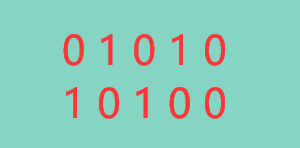
\includegraphics[width=0.5\textwidth]{problem4picture1}

	}
	由于$y$是$x$向高位移动产生的,所以一定是$y$的最高位为$1$,$x$此位为$0$,为了满足条件,需要向$a$和$b$的低位借位。
	
	我们首先思考什么情况不存在$a$,$b$满足条件。假设我们在某低位已经欠高位一位数了(俗称欠债):
	\begin{itemize}
		\item 当$x$此位为$0$时,我们可以使$a$、$b$都置1来向高位进位来还清债务,此时无论$y$是1还是0都有机会处理掉:如果是1的话,就相当于再向低位借位;如果是0的话,就已经满足条件了;
		\item 当$x$为$1$时,由于$a$+$b$一定为0+1的状态,所以靠这一位是没法还债的,只能依靠于下一位进位,才能加起来变成$10$,也就是说,这一位的和一定是$0$,此时,如果$y$要求1的话,便无法满足条件了。
	\end{itemize}
	\begin{corollary} 
		在已经被借位的情况下,$x=1$且$y=0$时$ab$不存在解。
		\label{cor-1}
	\end{corollary}
	“还债”的事情讨论完了,我们再讨论一下导致“欠债”的情况。
	\begin{itemize}
		\item 当$x$为$0$时,考虑到$ab$相同,相加的结果一定是$0$,所以当$y$等于1的时候会导致“欠债”,需要借位。
		\item 当$x$为$1$时,考虑到$ab$不同,结果一定是$1$,当$y$等于0时会导致“欠债”。
	\end{itemize}
	由此,可以得出答案。但是依靠分类讨论的解法,我们忽视了一个条件:$x$和$y$是错位的相同的,事实上,依靠这个条件,我们可以用一个更简单的结论去总结上述情况:
	
	\begin{corollary} 
		x中不能包含连续的1
		\label{cor-1}
	\end{corollary}
	
	考虑到:$x$和$y$是错位的相同的,那么$x$中连续的1一定会导致“欠债”状态下的$x=1,y=0$,或者是直到结尾也无法还债的情况$x=1,y=1$,所以一定不满足条件。
	
	\subsection{参考代码}
	\lstinputlisting[
	style       =   cpp,
	caption     =   {Vlad and a Pair of Numbers参考代码},
	label       =   {problem4.cpp}
	]{problem4.cpp}
\end{document}